\documentclass[graphics]{beamer}
\usepackage[english]{babel}
\usepackage[utf8]{inputenc}
\usepackage{tcolorbox}
\usepackage{pgfpages}
\usepackage{hyperref}

\setbeameroption{show notes}
\setbeameroption{show notes on second screen=right}

\usetheme{ENSLyon}

\title[Title]{Dicotomix}
\author[T.S]{M. Guy, E. Hazard, E. Kerinec, F. Lecuyer, P. Mangold,\\ A. Martin, R. Pellerin, N. Pinson, A. Slowik, T. Stérin}
\date{\today}

\setbeamersize{text margin left=20pt,text margin right=20pt}
\setbeamertemplate{navigation symbols}{}
\usecolortheme{ENSLyon_blue}
\addtobeamertemplate{navigation symbols}{}{
	\usebeamerfont{footline}
	\usebeamercolor[fg]{footline}
	\hspace{1em}
	\insertframenumber/\inserttotalframenumber
}

\begin{document}

\begin{frame}
	\titlepage
	\note{Speaker = Tristan}
	\begin{center}
		
\includegraphics[scale=0.2]{dicotomix}
		
\includegraphics[scale=0.08]{logoens}
		\hspace{2em}
		
\includegraphics[scale=0.55]{ars}
		\hspace{2em}
		
\includegraphics[scale=0.3]{hospices_civils_de_lyon}
	\end{center}
\end{frame}

\begin{frame}{Some figures about Dicotomix}
	\begin{itemize}
		\item 24 contributors
		\item 300 commits
		\item 50 hours meeting at ENS
		\item 30 hours meeting outside
		\item 2 hackathons
	\end{itemize}
\end{frame}

\section*{Content}
\begin{frame}
	\tableofcontents
\end{frame}

\section{Introduction}
\subsection{History}

\begin{frame}{The history of our project}
	\begin{itemize}
		\item Initial idea
		\begin{itemize}
			\item March 3rd 2016 : SIESTE by Maureen Clerc (BCI)
			\item Begining of September : using Akinator thanks to BCI in order to communicate
		\end{itemize}
		\pause
		\item November 2016 : Meeting with doctors
		\begin{itemize}
			\item November 19th : Alexandra Corneyllie lends us a BCI helmet
			\item November 18th to 20th : 1st Hackathon at ENS Lyon, we managed to make the hemlet work
			\item November 20th : Meeting a lot of people. Charlie who made the interface
		\end{itemize}
	\end{itemize}
\end{frame}

\begin{frame}{BCI (Brain Computer Interface)}
	\begin{center}
		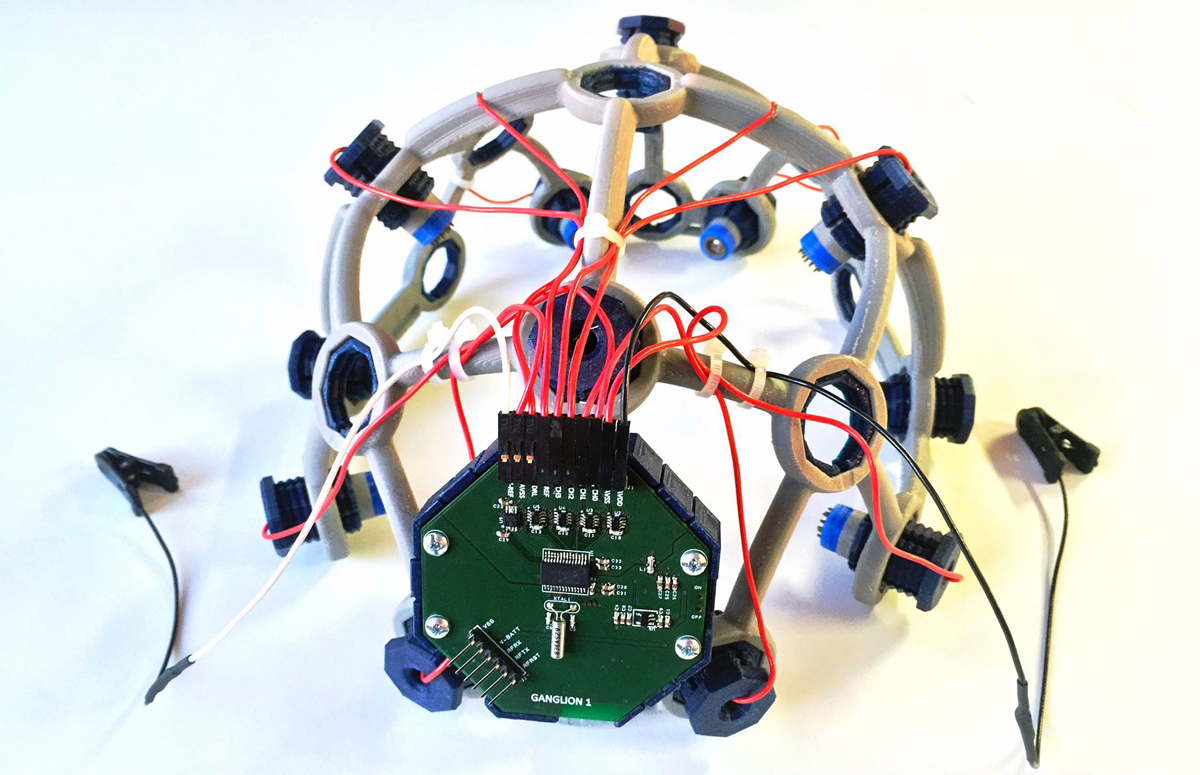
\includegraphics[scale=0.1]{bci}
		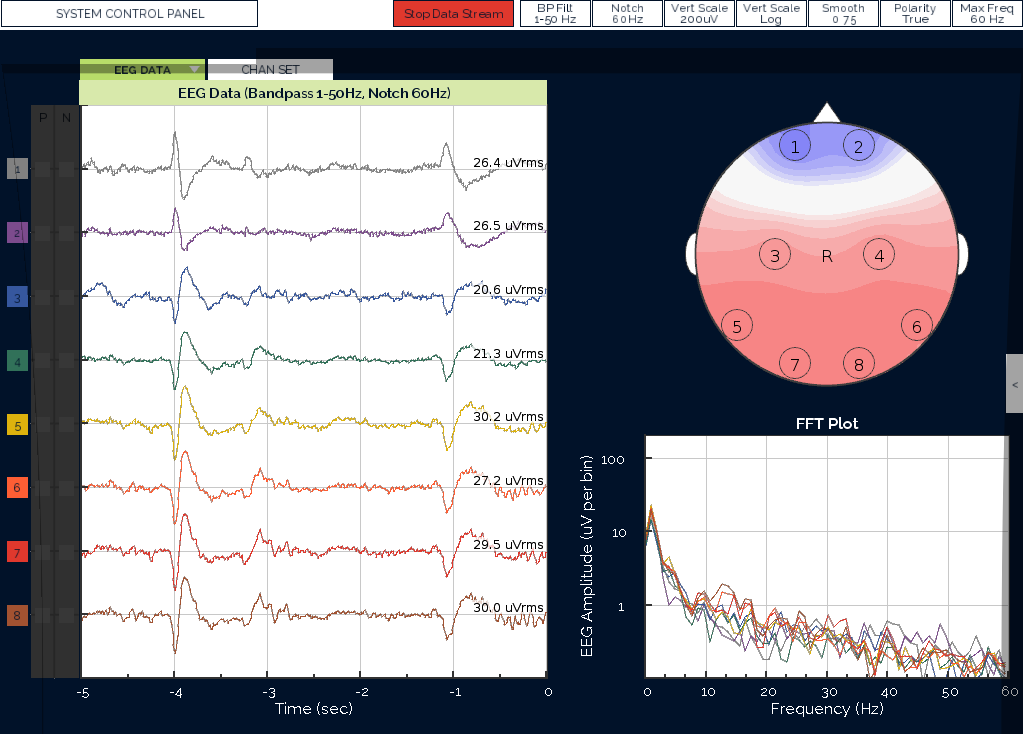
\includegraphics[scale=0.1]{openbci}
	\end{center}
	\begin{center}
		\begin{tcolorbox}[colback=green!5,colframe=green!40!black,title=Initial Idea]
			Use of BCI for people who cannot move anything.
			\note{This was our initial idea.}
		\end{tcolorbox}
		\pause
		\begin{tcolorbox}[colback=red!5,colframe=red!40!black,title=Reallity]
			Not only was it hard to get a good signal but also to deal with it afterwards!
			\note{We decided to make a break with BCI and to focus on the software part. But we are currently working on it again with Stephan Roux and Amine Metani (physicians at ENS Lyon).}
		\end{tcolorbox}
		\note{Talk about the first meeting with Luauté who tells us to stop working on BCI...}
	\end{center}
\end{frame}

\begin{frame}{History of our project 2}
	\begin{itemize}
		\item January 3rd 2017 : Meeting with Pr Luauté
		\begin{itemize}
			\item BCI is too complicated
			\item Our first idea of dichotomy is a good one !
			\item This could also be useful for the Charcot disease
		\end{itemize}
		\pause
		\item April 17th : Start of clinical trials
	\end{itemize}
\end{frame}

\begin{frame}{Quite a few people involved...}
	\begin{center}
		\vspace{-2cm}
		\hspace{-1cm}
		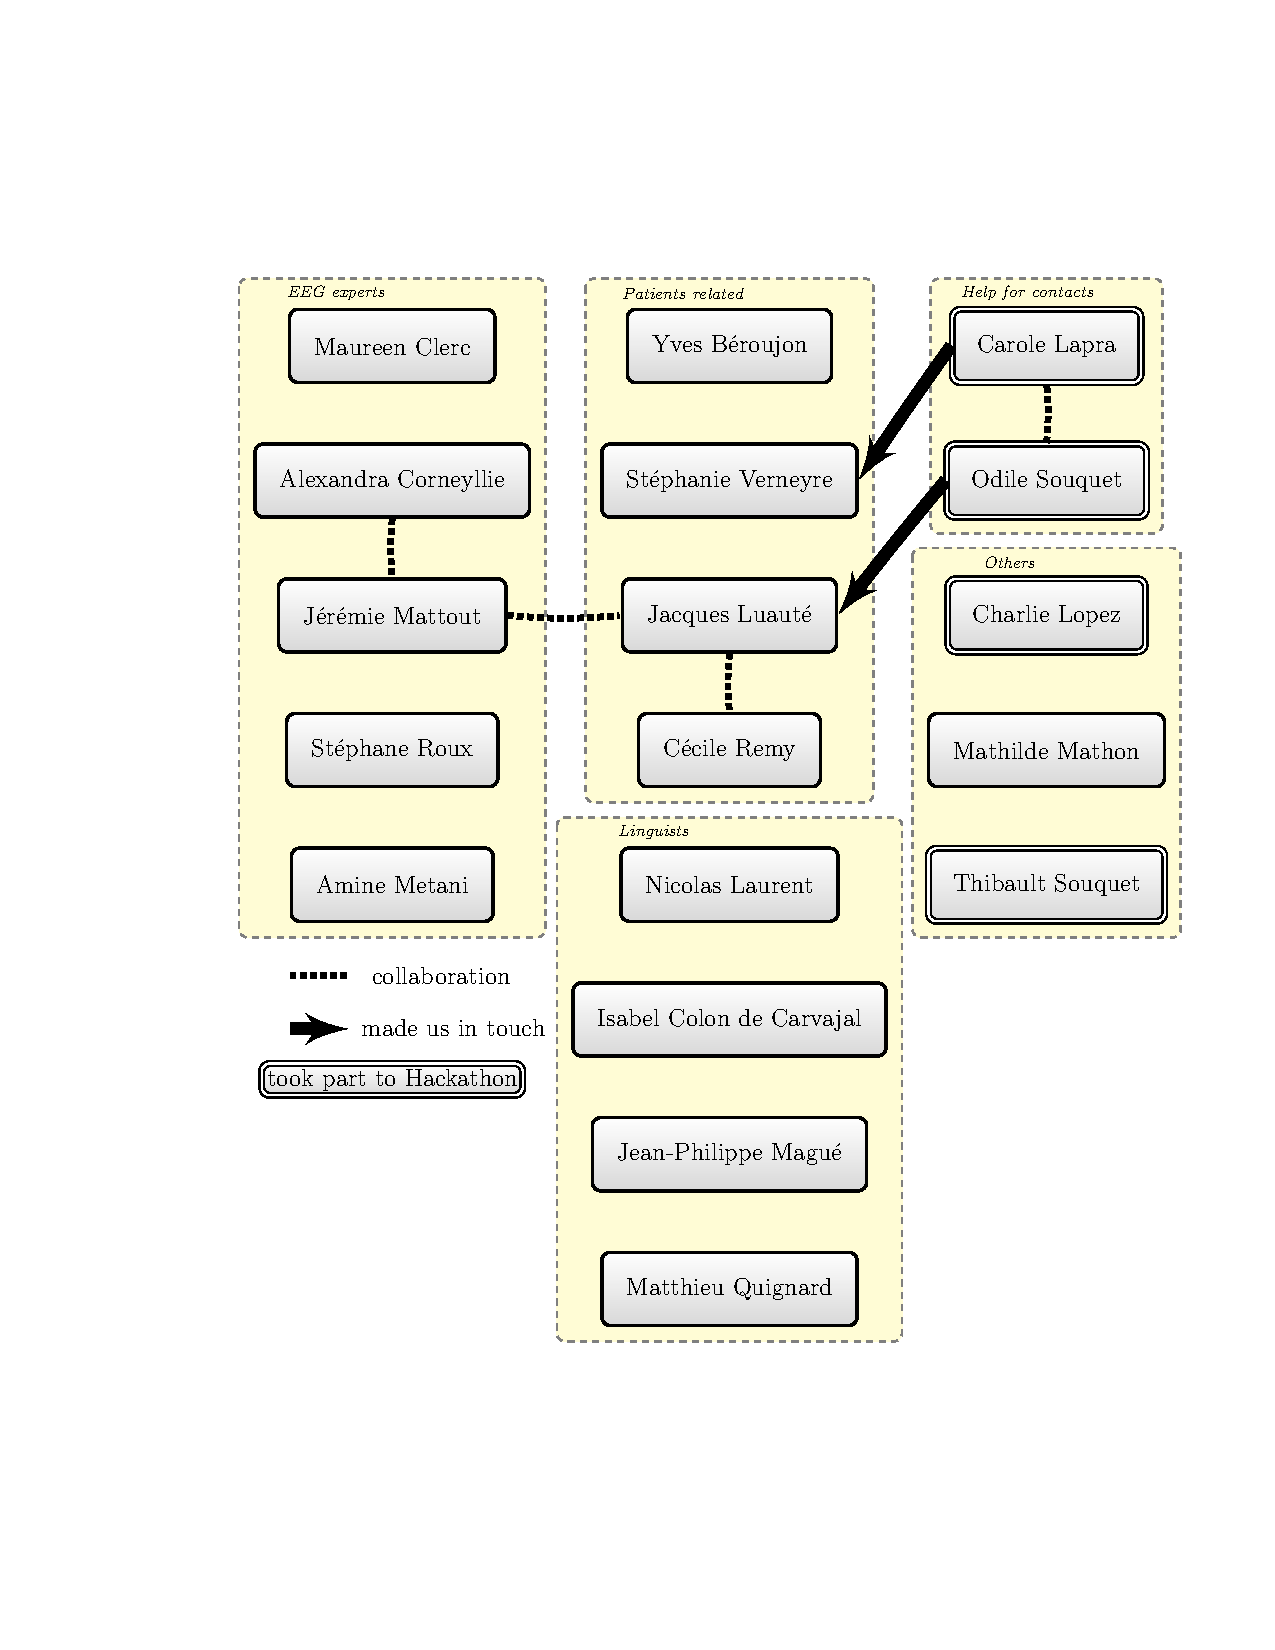
\includegraphics[scale=0.4]{graphe_intervenants.pdf}
	\end{center}
\end{frame}

\subsection{Motivations}

\begin{frame}{Charcot disease and locked-in syndrome}
	\note{Speaker = Nicolas}
	\begin{tcolorbox}[colback=red!5,colframe=red!40!black,title=Amyotrophic lateral sclerosis]
		Causes the death of motor neurons, and the gradual weakening of most muscles.
		\\
		6 000 cases in France, 150 000 in the world.
	\end{tcolorbox}
	\note{ALS is also called "maladie de Charcot"}
	\pause
	\begin{tcolorbox}[colback=red!5,colframe=red!40!black,title=Locked-In Syndrom]
	Different causes (often stroke), resulting on the unability to move most muscles, but keeping cognitive habilities.
	\\
	600 cases in France.
	\end{tcolorbox}
	
	\begin{center}
		\begin{itemize}
			\item People suffering are almost entirely paralized
			\item But they have all their cognitive abilities
		\end{itemize}
	\end{center}
\end{frame}

\subsection{Approach}

\begin{frame}{Existing methods : EJASINT}
	\begin{center}
		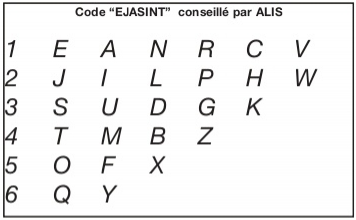
\includegraphics[scale=0.7]{ejasint}
	\end{center}
\end{frame}

\begin{frame}{Existing methods : ARS}
	\begin{center}
		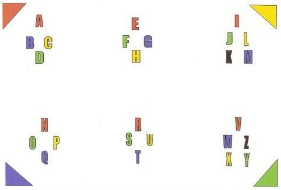
\includegraphics[scale=0.9]{tableau_lettres_transparent}
	\end{center}
\end{frame}

\begin{frame}{Existing methods : "Par-Lé-Si-Lab"}
	\begin{center}
		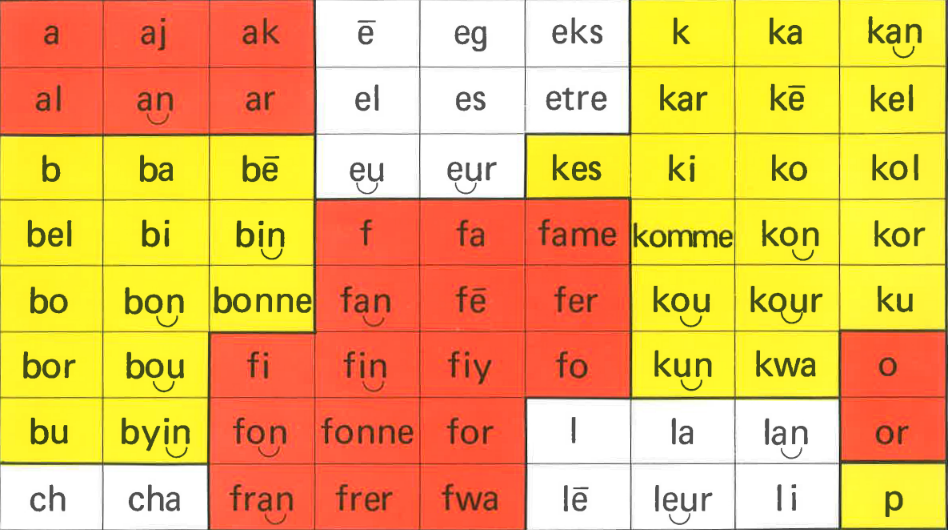
\includegraphics[scale=0.3]{parler_syllabes}
	\end{center}
\end{frame}

\section{The Dicotomix's original approach}
\subsection{The concept}

\begin{frame}{Concept}
	\begin{center}
		\begin{itemize}
			\item Writing word by word rather than spelling (reduce frustration)
			\item Optimizing each question
				\note[item]{First, we thought about using something like "Akinator".}
			\item Making it intuitive thanks to a simple interface
				\note[item]{We've worked with designers.}
			\item The only requirement is a binary input
				\note[item]{Our software is indenpent of the binary input.}
		\end{itemize}
	\end{center}
\end{frame}

\begin{frame}{Demo}
	\note{Speaker = Alexandre}
	\begin{center}
		
\includegraphics[scale=0.6]{aladdin}
	\end{center}
\end{frame}

\subsection{The algorithm}

\begin{frame}{The algorithm}
	\note{Speaker = Emile}
	\begin{center}
		\begin{itemize}
			\item Dichotomy over a dictionary (right/left signals)
			\item Frequencies of words taken into account
				\note[item]{Explainations on the board!}
			\item We can deduce the prefix and mark it green.
				\note[item]{This is espacially useful for error detection. We'll see later.}
		\end{itemize}
		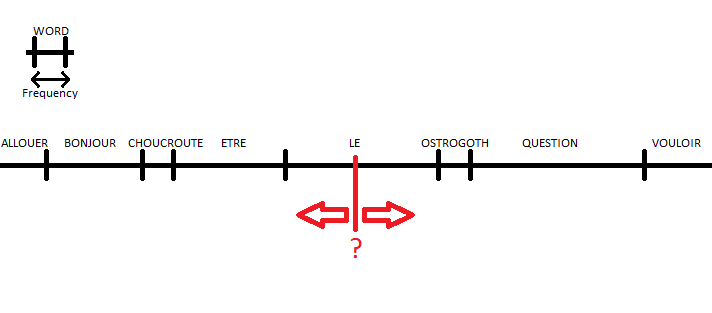
\includegraphics[scale=0.4]{algo}
	\end{center}
\end{frame}

\begin{frame}{Its implementation}
	\note{Speaker = Alexandre}
	\begin{itemize}
		\item The UI was developed with web technologies only
		\pause
		\item HTML/CSS for the graphical part
		\pause
		\item NodeJS for the logical part
		\pause
		\item Can run on many platforms
	\end{itemize}
\end{frame}

\subsection{Ergonomy}

\begin{frame}{But is Dicotomix really faster ?}
	\note{Speaker = Rémi}
	\begin{center}
		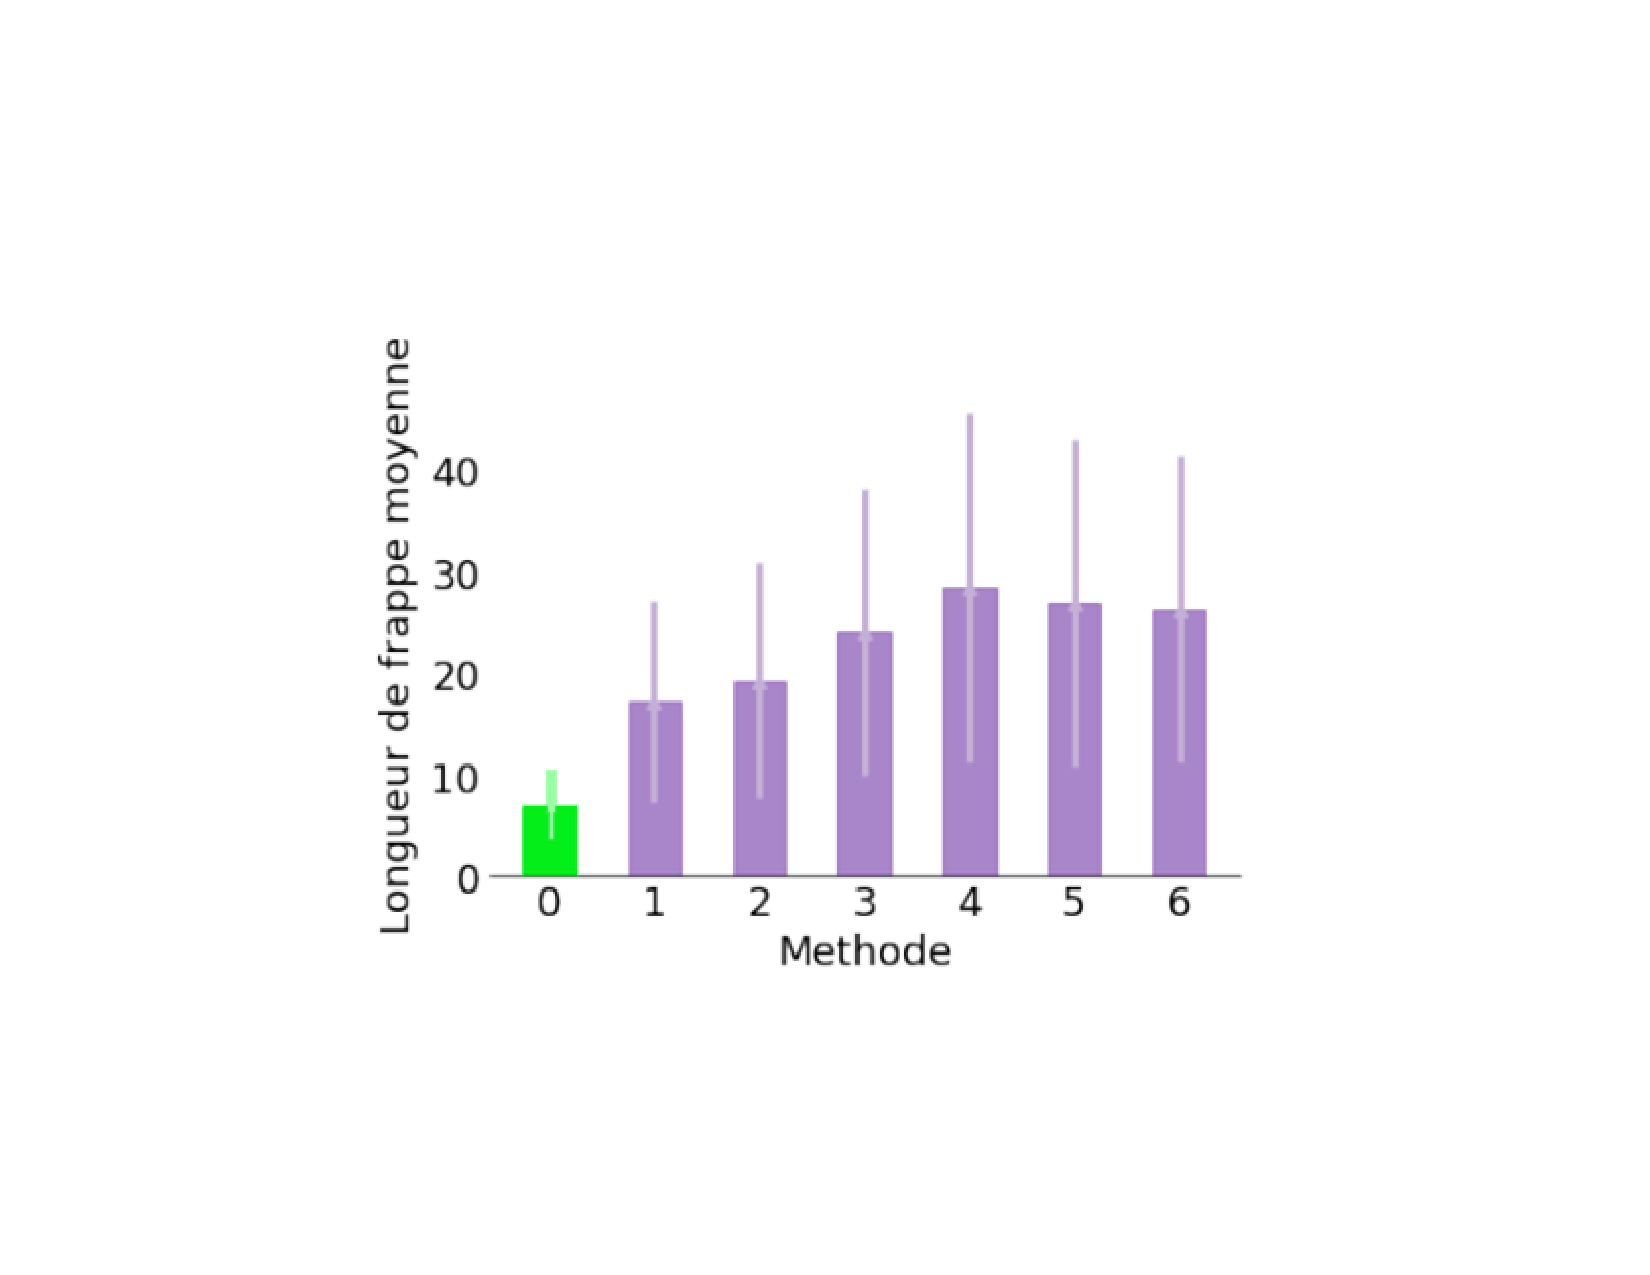
\includegraphics[scale=0.35]{graphe_comparatif.pdf}
	\end{center}
\end{frame}

\begin{frame}{Assets / Drawbacks}
	\begin{tcolorbox}[colback=green!5,colframe=green!40!black,title=Assets]
		\begin{itemize}
			\item Faster than spelling
				\note[item]{We made a comparison between some existing methods and ours. This could also be proved theoretically.}
			\item One can get better by training
				\note[item]{This will be confirmed by the study.}
			\item Could even have some fun playing with Dicotomix!
				\note[item]{The user is not as passive as in the methods described before.}
		\end{itemize}
	\end{tcolorbox}
	\pause
	\begin{tcolorbox}[colback=red!5,colframe=red!40!black,title=Drawbacks]
		\begin{itemize}
			\item It's hard to deal with mistakes
			\item Counterintuitive at the beginning (requires some training)
			\item Requires to be really focused
			\item What about proper names ?
		\end{itemize}
	\end{tcolorbox}
\end{frame}

\begin{frame}{How to deal with mistakes ?}
	\begin{itemize}
		\item Cannot automatically correct mistakes
			\note[item]{What is the patient is wrong on the first letter ?}
		\pause
		\item How to discard the last choice ?
			\note[item]{We've implemented it, we will show you next.}
		\pause
		\item How to edit the current sentence ?
			\note[item]{Currently, Dicotomix aimed to be used in everyday life, not for writing a book!}
		\pause
		\item Can we deal with semantic mistakes ?
	\end{itemize}
\end{frame}

\begin{frame}{Demo (strikes back!)}
	\note{Speaker = Alexandre}
	\begin{center}
		
\includegraphics[scale=0.6]{aladdin2}
	\end{center}
\end{frame}

%\begin{frame}{The ergonomy of Dicotomix}
%	\begin{center}
%		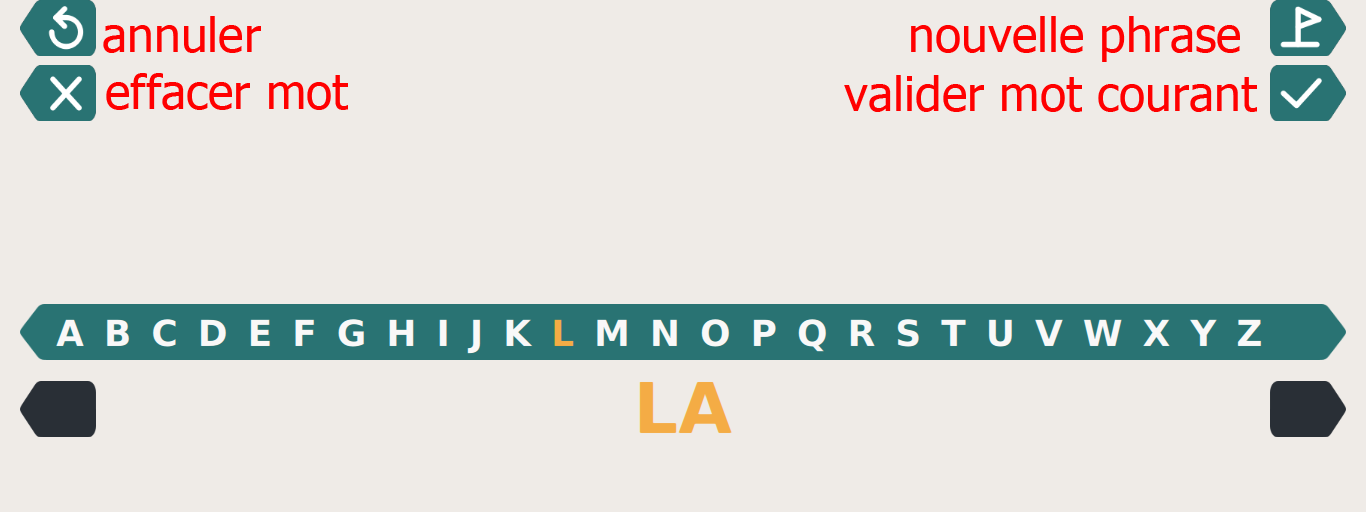
\includegraphics[scale=0.2]{vierge}
%	\end{center}
%\end{frame}

%\begin{frame}{The ergonomy of Dicotomix 2}
%	\begin{center}
%		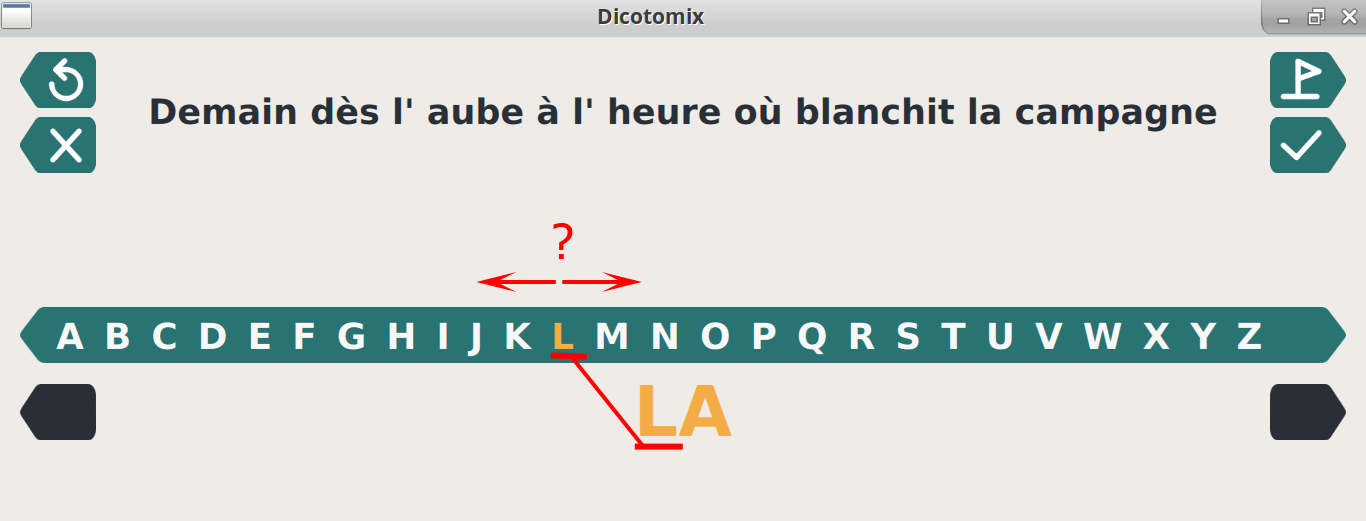
\includegraphics[scale=0.2]{example1}
%	\end{center}
%\end{frame}

%\begin{frame}{The ergonomy of Dicotomix 3}
%	\begin{center}
%		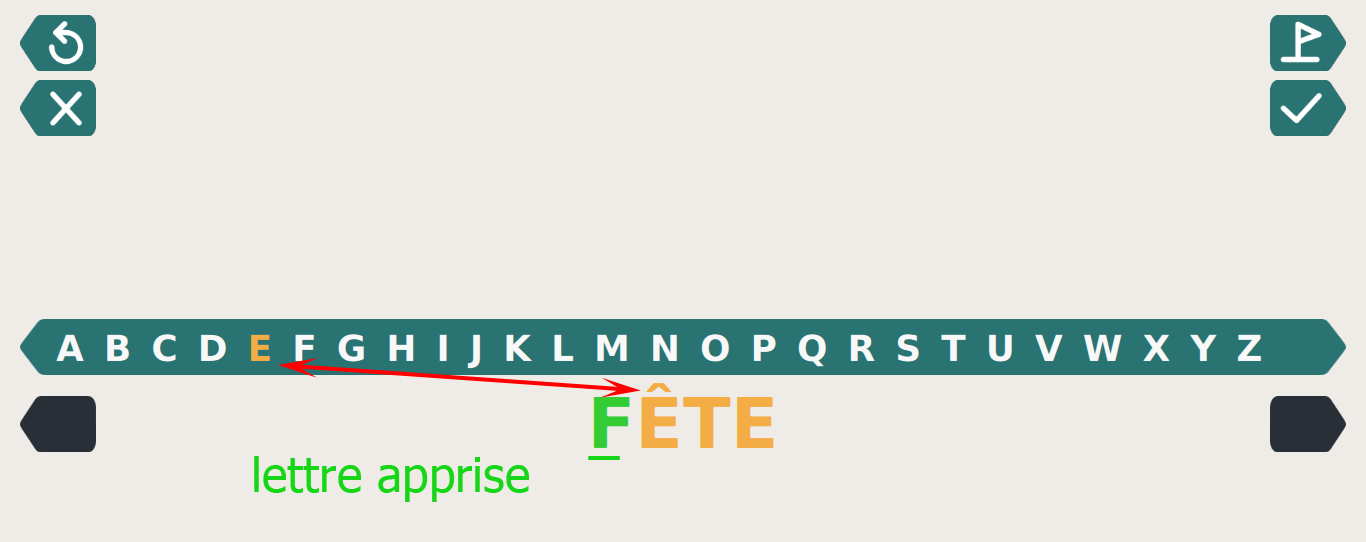
\includegraphics[scale=0.2]{encours}
%	\end{center}
%\end{frame}

\section{What's next ?}

\subsection{What remains to be done ?}

\begin{frame}{What remains to be done ?}
	\note{Speaker = Fabrice ?}
	\begin{center}
		\begin{itemize}
			\item Use of every possible dictionary
			\item Possibility to change frequencies using some heuristics
			\item Adaptation to the patient
		\end{itemize}
	\end{center}
\end{frame}

\subsection{Test phase}

\begin{frame}{Clinical trials}
	\begin{center}
		\begin{itemize}
			\item Hôpital Neurologique Pierre Wertheimer
				\note[item]{starting next week}
			\item A few patients
			\item A training phase and an evaluation phase
		\end{itemize}
	\end{center}
\end{frame}


%\begin{frame}{Test protocol}
%	A training session:
%	\begin{itemize}
%		\item 10 words to find using Dicotomix
%		\item Spell a name
%		\item 3 questions
%		\item Free talk ("Do you want to say anything?")
%	\end{itemize}
%	Evaluation: write a text using Dicotomix, then the usual method
%\end{frame}

\begin{frame}{Example of a test session}
	\note{Speaker = Tristan}
	\begin{enumerate}
		\item Try to find the following words :
			\begin{itemize}
			\item présents
			\item tout
			\item philosophie
			\item clochette
			\item fichus
			\item co-animateur
			\item anthracine
			\item cyclorama
			\item polymorphes
			\item géothermale
		\end{itemize}
	\pause
	\item Spell, using the spelling mode, the proper name you want.
	\pause
	\item Ask 3 questions.
	\pause
	\item Free talk.
	\end{enumerate}
	Then we evaluate
\end{frame}

\begin{frame}{Protocol and evaluation}
	\begin{itemize}
		\item Training phase to become familiar with the method
			\note[item]{To allow more revelance when you compare to the usual method during the test phase.}
		\item Several session to measure the speed of progress in using the method
		\item Measure the difference in their speeking during the time
			\note[item]{more complex phrases, use of pronoms...}
		\item Know their feeling about Dicotomix, and if they want to continue to use it
			\note[item]{if they are comfortable with it and how it evolves, if they want to use it when they are familiar and not discovering it}
	\end{itemize}
\end{frame}
\subsection{Distribution}
\begin{frame}{Reaching patients}
	\hspace{7cm}
	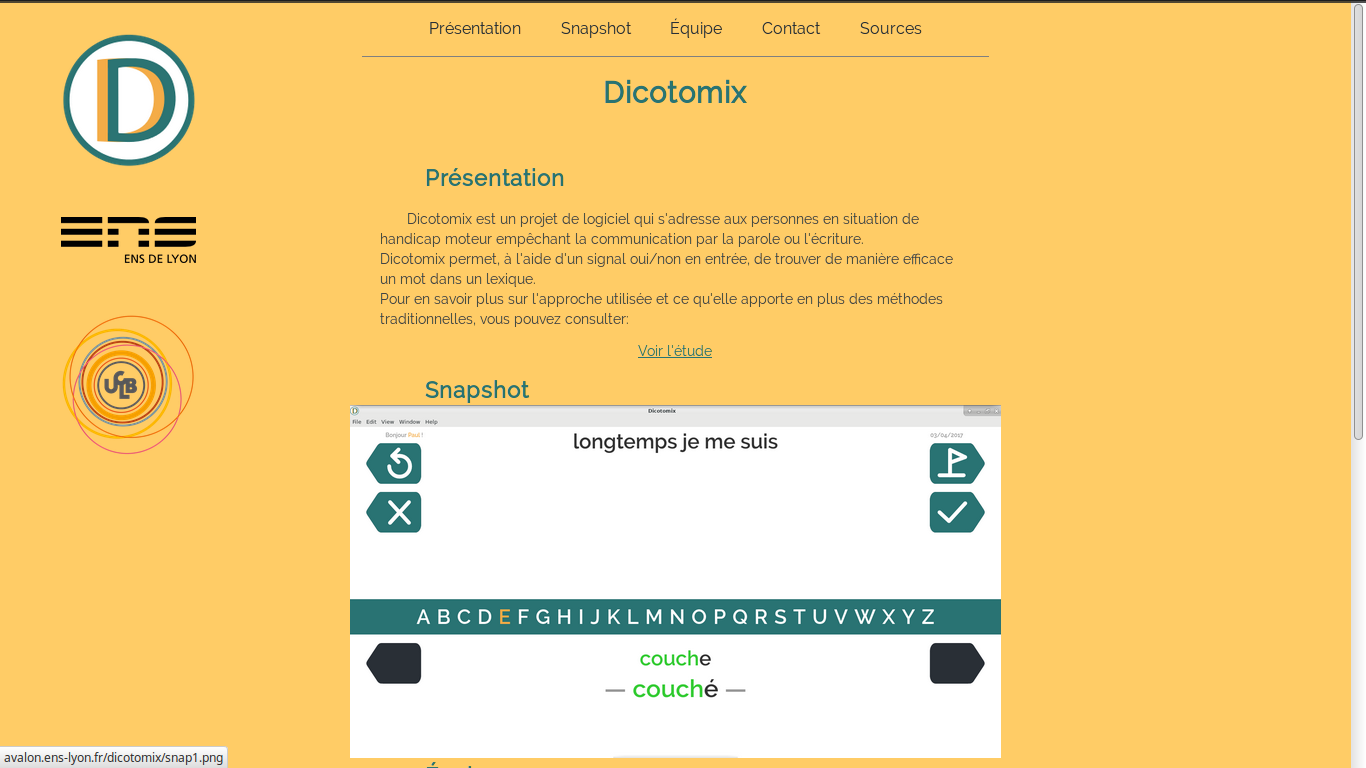
\includegraphics[scale=0.075]{website}\\
	\begin{itemize}
		\item Help of metropole de Lyon and ARSLA
			\note[item]{With possibily other partners...}
		\item The code is available on our website : \hyperref[http://avalon.ens-lyon.fr/dicotomix]{http://avalon.ens-lyon.fr/dicotomix}
		\item As well as on GitHub
		\item A Tutorial is available
	\end{itemize}
	\hspace{10cm}
	
\includegraphics[scale=0.07]{opensource}
\end{frame}

\begin{frame}{Questions ?}
	\begin{center}
		Thank you for your attention!
		\begin{center}
			\begin{picture}(100,100)
				\put(15,30){
\includegraphics[scale=0.2]{dicotomix}}
				\put(-15,50){
\includegraphics[scale=0.2]{ars}}
				\put(55,-25){
\includegraphics[scale=0.1]{alis}}
				\put(90,30){
\includegraphics[scale=0.1]{arsla}}
				\put(30,80){
\includegraphics[scale=0.05]{logoens}}
				\put(-15,0){
\includegraphics[scale=0.2]{hospices_civils_de_lyon}}
			\end{picture}
		\end{center}
		\vspace{1cm}
		Special thanks to all our contacts!
	\end{center}
\end{frame}
\end{document}
